\documentclass[12pt]{article}

\usepackage{sbc-template}
\usepackage{graphicx,url}
\usepackage[utf8]{inputenc}
\usepackage[brazil]{babel}
\usepackage{lipsum}
%\usepackage[latin1]{inputenc}  
\usepackage{amsmath}
\usepackage[portuguese,ruled,vlined]{algorithm2e}
%\usepackage[portuguese,ruled,vlined,linesnumbered]{algorithm2e}
     
\sloppy

\title{Componentes Conexos em Processador Multicore}
\author{Patreze A. Chita \inst{1}, Nahri. B. Moreano\inst{1}}
\address{Faculdade de Computação -- Universidade Federal do Mato Grosso do Sul (UFMS) \\ Caixa Postal 549 -- 79.070.900 -- Campo Grande -- MS -- Brazil
\email{patrezechita@gmail.com, nahri@facom.ufms.br}
}

\begin{document} 

\maketitle

\begin{abstract}
  This meta-paper describes the style to be used in articles and short papers
  for SBC conferences. For papers in English, you should add just an abstract
  while for the papers in Portuguese, we also ask for an abstract in
  Portuguese (``resumo''). In both cases, abstracts should not have more than
  10 lines and must be in the first page of the paper.
\end{abstract}
     
\begin{resumo} 
  Este meta-artigo descreve o estilo a ser usado na confecção de artigos e
  resumos de artigos para publicação nos anais das conferências organizadas
  pela SBC. É solicitada a escrita de resumo e abstract apenas para os artigos
  escritos em português. Artigos em inglês deverão apresentar apenas abstract.
  Nos dois casos, o autor deve tomar cuidado para que o resumo (e o abstract)
  não ultrapassem 10 linhas cada, sendo que ambos devem estar na primeira
  página do artigo.
\end{resumo}

\section{Introdução}
\lipsum[1]

\section{Algoritmo Sequencial e Paralelo para Componentes Conexos}
\lipsum[1]
\subsection{Algoritmo Sequencial Baseado em Busca em Profundidade}

algoritmo 1.

\begin{algorithm}
    \DontPrintSemicolon
    \caption{Implementação do Algoritmo Sequencial para C. C.}
    \SetKwProg{ComponentesConexos}{sequencialDFS}{}{}
    \ComponentesConexos{$(G=(V,\ A))$}
	{
        $nComponente \gets 0$\;
        $visitado[v] \gets FALSO \mid \forall v \in V$\;
        %$visitado[v] \gets FALSO,\ \{ \forall\ v \mid v \in V\}$\;
        %\ParaCada{$v\acute{e}rtice\ u \in V$}
        %{
        %    $visitado[u] \gets FALSO$\;
        %}
    
        \ParaCada{$v\acute{e}rtice\ v \in V$}
        {
            \Se{$visitado[v] = FALSO$}
            {
                $\textbf{DFS}(v)$\;
                $nComponente \gets nComponente + 1$\;
            }
        }
    }
    
    \SetKwProg{DFS}{DFS}{}{}
    \DFS{$(v\acute{e}rtice\ v)$}
    {
        $componente[v] \gets nComponente$\; 
        $visitado[v] \gets VERDADEIRO$\;
        \ParaCada{$v\acute{e}rtice\ u \in Adj[v]$}
        {
            \Se{$visitado[u] = FALSO$}
            {
                $\textbf{DFS}(u)$\;
            }
        }
    }
\end{algorithm}

\subsection{Algoritmo Paralelo Baseado em Busca em Profundidade e nas Operações Union/Find}

algoritmo 2.

\begin{algorithm}
    \DontPrintSemicolon
    \caption{Algoritmo Paralelo para C. C.}
    %\caption{Componentes conexos -- Paralelo \cite[gramma]}
    \SetKwProg{ComponentesConexosPar}{paraleloGrama}{}{}
    \ComponentesConexosPar{$(G=(V,E))$}
    {
        $p \gets$ número de processadores\;
        Divide vértices de $V$ em $p$ partes de $\sim|V|/p$ vértices\;
        \ParaCada{processador $p_i$ em paralelo}
        {
            $V_i \gets$ vértices de $V$ alocados a $p_i$\;
            $G_i \gets$ subgrafo de $G$ induzido por $V_i$\;
            Realiza DFS($G_i$) produzindo floresta $F_i$\;
        }

        Une florestas $F_i$, par a par, em paralelo, produzindo floresta $F$\;
        
        \tcp{Para cada árvore $A$ $\in$ $F$, vértices de $A$ estão no mesmo componente}
    }
\end{algorithm}

\section{Solução Paralela para Componentes Conexos para Processador Multicore}

\begin{algorithm}
    \DontPrintSemicolon
    \caption{Implementação do Algoritmo Paralelo para C. C.}
    \SetKwProg{ComponentesConexosPar}{paraleloPatreze}{}{}
    \SetKwFor{ForPar}{para cada}{fa\c{c}a em paralelo}{fim para cada}
    \SetKw{Return}{retorna}
    \ComponentesConexosPar{$(G=(V,A))$}
    {
        $nTh \gets n\acute{u}mero\ de\ threads$\;

        \Para{$t \gets 0\ \Ate\ (nTh - 1)$}
        {
        	%$verticeInicial[t] \gets t \times (\sim \frac{|V|}{nTh})$\;
        	%$verticeFinal[t] \gets verticeInicial[t] + (\sim \frac{|V|}{nTh})-1$\;
        	$verticeInicial[t] \gets t \times \lfloor \frac{|V|}{nTh} \rceil$\;
        	$verticeFinal[t] \gets verticeInicial[t] + \lfloor \frac{|V|}{nTh} \rceil-1$\;
        }
        
        %$nVerticeExtra \gets |V| - (\lfloor \frac{|V|}{nTh} \rfloor \times nTh)$\;
        %\Para{$t \gets 0$ \Ate $(nTh-1)$}
        %{
        %    \eSe{$t < $nVerticeExtra}
        %    {
        %        $verticeInicial[t] \gets t \times \lceil \frac{|V|}{nTh} \rceil$\;
        %        $verticeFinal[t] \gets verticeInicial[t] + \lceil \frac{|V|}{nTh} \rceil - 1$\;
        %    }
        %   {
        %        $verticeInicial[t] \gets t \times \lfloor \frac{|V|}{nTh} \rfloor + nVerticeExtra$\;
        %        $verticeFinal[t] \gets verticeIncial[t] + \lfloor \frac{|V|}{nTh} \rfloor - 1$\;
        %    }
        %}
        
        %\tcp{Realiza DFS em paralelo}
        %$inicializa\ compnente[][]$\;
        \ForPar{$t \gets 0\ \Ate\ (nTh - 1)$}
        {
        
            %\ParaCada{vértice $v \in V$}
            %{
            %    $componente[t][v] \gets v$\;
            %}
            $componente[t][v] \gets v \mid \forall v \in V$\;
            $floresta[t] \gets \emptyset$\;
            \Para{$v\gets verticeInicial[t]\ \Ate\ verticeFinal[t]$}
            {
                \Se{$visitado[v] = FALSO$}
                {
                    $raiz \gets v$\;
                    $\textbf{DFS}(t,\ v,\ raiz)$\;
                }
            }
        }
        
        %\tcp{Une florestas para a par em paralelo}
        $nPares \gets \frac{nTh}{2}$\;
        \Para{$i \gets 0\ \Ate\ (\log_2(nTh)-1)$}
        {
            %\tcp{EXECUÇÃO UNION-FIND EM PARALELO}
            \ForPar{$t \gets 0\ \Ate\ (nPares-1)$}
            {
                $thEsq \gets t \times 2^{i+1}$\;
                $thDir \gets thEsq + 2^i$\;
                
                \ParaCada{$(v,\ u) \in floresta[thDir]$}
                {
                    $\textbf{UNION}(thEsq,\ v,\ u)$\;
                }
            }
            $nPares \gets \frac{nPares}{2}$\;
        }
    }
    \SetKwProg{DFS}{DFS}{}{}
    \DFS{$(thread\ t,\ v\acute{e}rtice\ v,\ raiz)$}
    {
        $componente[t][v] \gets raiz$\;
        
        \ParaCada{$v\acute{e}rtice\ u \in Adj[v]$}
        {
            $floresta[t] \gets floresta[t] \cup (v,\ u)$\;
            $componente[t][u] \gets raiz$\;
            
            \Se{$verticeInicial[t] \le u \le verticeFinal[t]$}
            {
                \Se{$visitado[u] = FALSO$}
                {
                    $\textbf{DFS}(t,\ u,\ raiz)$\;
                }
            }
        }
        $visitado[v] \gets VERDADEIRO$\;
    }
    \SetKwProg{UNION}{UNION}{}{}
    \UNION{$(thread\ t,\ v\acute{e}rtice\ v,\ v\acute{e}rtice\ u)$}
    {
        $fV \gets  \textbf{FIND}(t,\ v)$\;
        $fU \gets  \textbf{FIND}(t,\ u)$\;
        
        \Se{$fV \neq fU$}
        {
            \Para{$i \gets 0\ \Ate\ (|V|-1)$}
            {
                \Se{$componente[t][i] = fV$ \textbf{ou} $componente[t][i] = fU$}
                {
                    $componente[t][i] \gets \textbf{M} \acute{\textbf{I}} \textbf{NIMO}(fV,\ fU)$\;
                }
            }
            $floresta[t] \gets floresta[t] \cup (v,\ u)$\;
        }
    }
    \SetKwProg{FIND}{FIND}{}{}
    \FIND{$(thread\ t,\ v\acute{e}rtice\ v)$}
    {
        \Return $componente[t][v]$\;
    }
\end{algorithm}

\begin{figure}
\centering
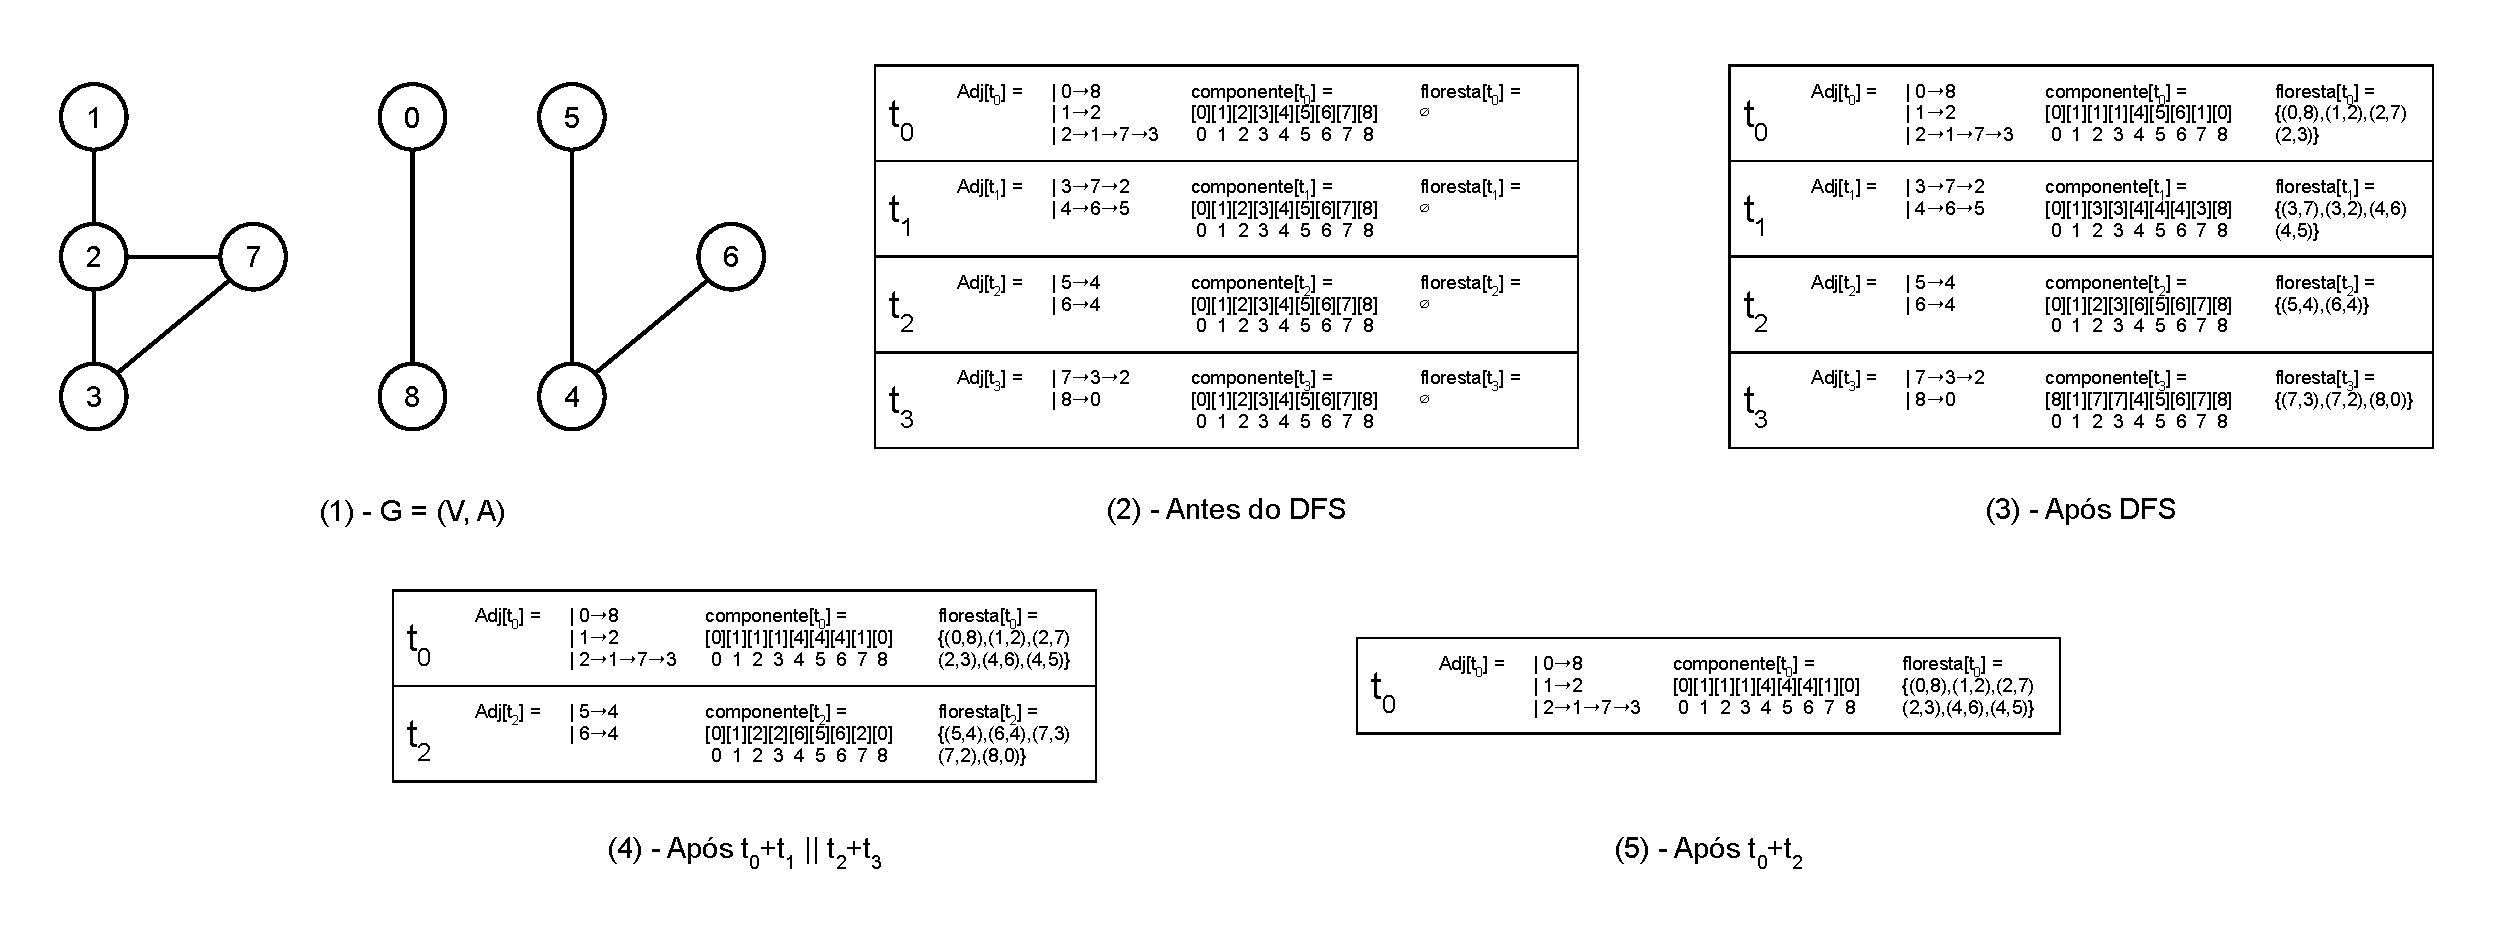
\includegraphics[width=1\textwidth]{tabela_exe_par.pdf}
\caption{Exemplo de Execução do Algoritmo 3}
\label{fig:alg3}
\end{figure}

\section{General Information}

All full papers and posters (short papers) submitted to some SBC conference,
including any supporting documents, should be written in English or in
Portuguese. The format paper should be A4 with single column, 3.5 cm for upper
margin, 2.5 cm for bottom margin and 3.0 cm for lateral margins, without
headers or footers. The main font must be Times, 12 point nominal size, with 6
points of space before each paragraph. Page numbers must be suppressed.

Full papers must respect the page limits defined by the conference.
Conferences that publish just abstracts ask for \textbf{one}-page texts.

\section{First Page} \label{sec:firstpage}

The first page must display the paper title, the name and address of the
authors, the abstract in English and ``resumo'' in Portuguese (``resumos'' are
required only for papers written in Portuguese). The title must be centered
over the whole page, in 16 point boldface font and with 12 points of space
before itself. Author names must be centered in 12 point font, bold, all of
them disposed in the same line, separated by commas and with 12 points of
space after the title. Addresses must be centered in 12 point font, also with
12 points of space after the authors' names. E-mail addresses should be
written using font Courier New, 10 point nominal size, with 6 points of space
before and 6 points of space after.

The abstract and ``resumo'' (if is the case) must be in 12 point Times font,
indented 0.8cm on both sides. The word \textbf{Abstract} and \textbf{Resumo},
should be written in boldface and must precede the text.

\section{CD-ROMs and Printed Proceedings}

In some conferences, the papers are published on CD-ROM while only the
abstract is published in the printed Proceedings. In this case, authors are
invited to prepare two final versions of the paper. One, complete, to be
published on the CD and the other, containing only the first page, with
abstract and ``resumo'' (for papers in Portuguese).

\section{Sections and Paragraphs}

Section titles must be in boldface, 13pt, flush left. There should be an extra
12 pt of space before each title. Section numbering is optional. The first
paragraph of each section should not be indented, while the first lines of
subsequent paragraphs should be indented by 1.27 cm.

\subsection{Subsections}

The subsection titles must be in boldface, 12pt, flush left.

\section{Figures and Captions}\label{sec:figs}


Figure and table captions should be centered if less than one line
(Figure~\ref{fig:exampleFig1}), otherwise justified and indented by 0.8cm on
both margins, as shown in Figure~\ref{fig:exampleFig2}. The caption font must
be Helvetica, 10 point, boldface, with 6 points of space before and after each
caption.

\begin{figure}[ht]
\centering
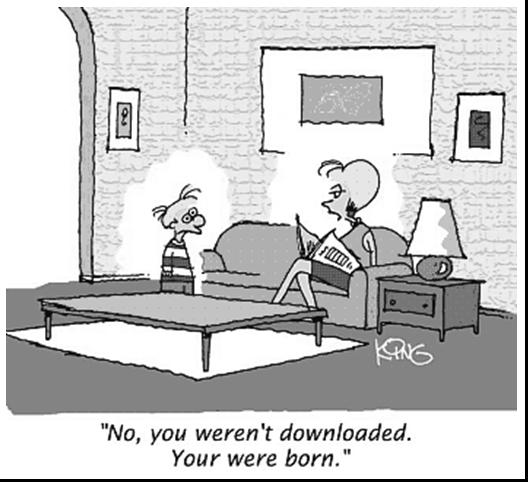
\includegraphics[width=.5\textwidth]{fig1.jpg}
\caption{A typical figure}
\label{fig:exampleFig1}
\end{figure}

\begin{figure}[ht]
\centering
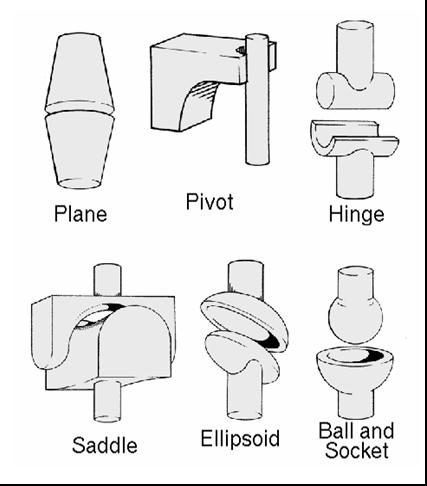
\includegraphics[width=.3\textwidth]{fig2.jpg}
\caption{This figure is an example of a figure caption taking more than one
  line and justified considering margins mentioned in Section~\ref{sec:figs}.}
\label{fig:exampleFig2}
\end{figure}

In tables, try to avoid the use of colored or shaded backgrounds, and avoid
thick, doubled, or unnecessary framing lines. When reporting empirical data,
do not use more decimal digits than warranted by their precision and
reproducibility. Table caption must be placed before the table (see Table 1)
and the font used must also be Helvetica, 10 point, boldface, with 6 points of
space before and after each caption.

\begin{table}[ht]
\centering
\caption{Variables to be considered on the evaluation of interaction
  techniques}
\label{tab:exTable1}
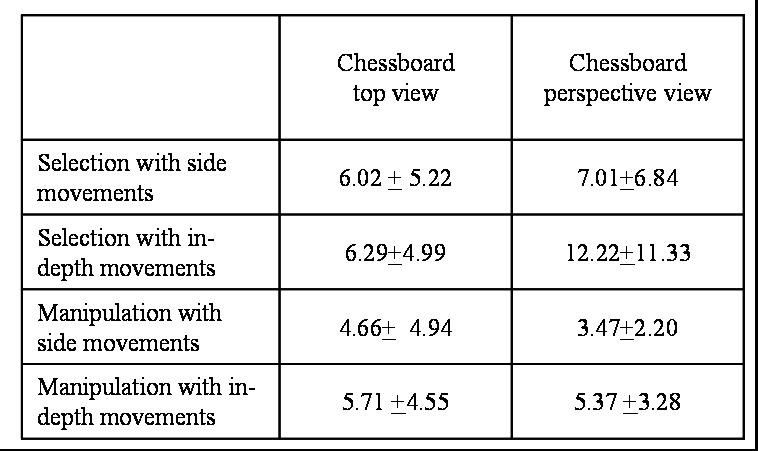
\includegraphics[width=.7\textwidth]{table.jpg}
\end{table}

\section{Images}

All images and illustrations should be in black-and-white, or gray tones,
excepting for the papers that will be electronically available (on CD-ROMs,
internet, etc.). The image resolution on paper should be about 600 dpi for
black-and-white images, and 150-300 dpi for grayscale images.  Do not include
images with excessive resolution, as they may take hours to print, without any
visible difference in the result. 

\section{References}

Bibliographic references must be unambiguous and uniform.  We recommend giving
the author names references in brackets, e.g. \cite{knuth:84},
\cite{boulic:91}, and \cite{smith:99}.

The references must be listed using 12 point font size, with 6 points of space
before each reference. The first line of each reference should not be
indented, while the subsequent should be indented by 0.5 cm.

\bibliographystyle{sbc}
\bibliography{sbc-template}

\end{document}
